\section{Propagazione guidata}%
Le equazioni delle onde piane uniformi trovate sinora si possono quindi applicare anche per la propagazione di onde elettromagnetiche in conduttori, per esempio
\begin{itemize}%
  \item \textbf{linee bifilari} come il doppino telefonico
  \item \textbf{linee coassiali}, per esempio  cavo che collega l'antenna al televisore
  \item \textbf{le guide rettangolari}, usate principalmente per applicazioni in cui è necessario trasportare molta potenza (radar o trasmissioni satellitari)
  \item \textbf{le linee a microstriscia} utilizzate per trasportare segnali in circuiti stampati
\end{itemize}
Accenniamo ora come si propaga l'onda in alcune di queste guide, poiché il segnale prima di essere emesso dall'antenna dovrà essere trasportato in una qualche maniera.
\paragraph{Campi nella guida}

I campi elettromagnetici che si propagano in guide d'onda il vettore di propagazione  e l'impedenza d'onda sono:
\begin{esp}
  |\k| &=\beta= \omega \sqrt{\mu \epsilon} \\
  \eta &= \frac{E_o}{H_o} = \sqrt{\frac{\mu}{\epsilon}}
\end{esp}

\paragraph{Linea bifilare}
Le linee di forza del campo elettrico nella linea bifilare sono simili a quelle di un condensatre, ossia $\forall$ punto $\E\perp\H\perp\k$. In figura \#TODO\# sono rappresentate le linee di campo.

\paragraph{Linea coassiale}
In questo caso le linee di campo elettrico sono ortogonali alla circonferenza, mentre quelle di campo magnetico sono concentriche all'asse della linea, come visibile in fig \#TODO\#

\paragraph{Impedenza caratteristica}
Cerchiamo ora di valutare l'impedenza caratteristica della linea e, in particolare, come sfruttarla per ridurre al minimo le perdite.

La tensione e la corrente nella linea coassiale si possono scrivere come
\begin{esp}
  V&= \int_{r_{int}}^{r_{ext}} \E \cdot d\vec{l} \\
  I&= \oint \H \cdot d\vec{l} \\
  &\implies Z_C = \frac{V_o}{I_o} \text{ impedenza caratteristica della linea}
\end{esp}
Definendo inoltre
\begin{itemize}
  \item $l$ l'induttanza per unità di lunghezza $\frac{H}{m}$
  \item $c$ la capacità per unità di lunghezza $\frac{F}{m}$
\end{itemize}
si ottiene che l'impedenza caratteristica risulta
\begin{equation}
  Z_C = \sqrt{\frac{l}{c}} = \underbrace{F_{forma}}_{\text{fattore di forma}} \cdot \sqrt{\frac{\mu}{\epsilon}}
\end{equation}

Possiamo quindi riscrivere le equazioni per la tensione e la corrente nel cavo coassiale come
\begin{esp}
  V(z) &= V_o \cdot e^{-\jmath \beta \cdot z}\\
  I(z) &= I_o \cdot e^{-\jmath \beta \cdot z}
\end{esp}


\chapter{Antenne}
In questo capitolo analizzeremo le antenne, partendo inizialmente con i potenziali elettromagnetici e cercando di modificare le equazioni di Maxwell affinché siano più comode da studiare nei nostri casi. Vedremo quindi l'equazione di Helmoltz e la scelta di Lorentz. Inizieremo quindi a studiare le antenne partendo dal caso del dipolo elementare, ideale e non realizzabile nella realtà, ma utile per fare le prime approssimazioni. Estenderemo quindi il dipolo elementare al dipolo corto per studiare poi le antenne lineari, le schiere e le patch.

Riprendiamo le equazioni di Maxwell scritte con i vettori di Steinmets:
\begin{equation}\label{eq:maxw-ant}\begin{cases}
  \rot\E = -\jmath \omega \mu\H(\r) \textcolor[rgb]{0.8,0,0}{+ \M} \\
  \rot\H = \jmath  \omega \epsilon \E + \J\\
  \diverg\H=0\\
  \diverg \E = \frac{\rho}{\epsilon}
\end{cases}\end{equation}
Ora aggiungiamo un termine $\M$ fittizio, affinché le equazioni risultino simmetriche e si possano scrivere, in seguito, le equazioni per le sorgenti equivalenti. ($\M$ non può esistere, in quanto non esiste il monopolo magnetico)

\subsubsection{Potenziali elettromagnetici}
$\forall \A , \diverg(\rot \A) = 0$ per quanto trovato nel paragrafo dell'identità notevole (\ref{sec:id-not}). Definiamo quindi $\A$  \textbf{potenziale vettore magnetico} il campo per cui $\H = \frac{1}{\mu} \cdot \rot \A$.
\paragraph{Teorema di Helmoltz}
Un campo vettoriale $\A$ è univocamente definito se sono fissati $\rot \A$ e $\diverg \A$
----------------

Dobbiamo dunque definire in maniera intelligente $\diverg \A$:
\begin{esp} \label{eq:AE}
  \rot\E &= - \jmath \omega \cdot \mu \frac{1}{\mu} \rot \A \quad \Leftrightarrow \quad \rot\left(\rot \E + \jmath \omega \A\right)=0 \\
  \forall \Phi& \text {, scalare, } \rot(\diverg\Phi)=0\\
  \E +& \jmath \omega \A = -\nabla\Phi \quad \implies \E = -\jmath \omega \A - \nabla \Phi  \\
  \implies &[\Phi] = V
\end{esp}
Definiamo quindi $\Phi$ potenziale scalare elettrico associato ad $\A$. Analizziamo ora la seconda equazione di Maxwell
\begin{esp}
  \rot \H &= \jmath \omega \epsilon_c \cdot \E + \J =  \mu \cdot \rot\left(\frac{1}{\mu} \rot \A\right)\\
   &= \jmath \omega \mu \epsilon_c \cdot \left(-\jmath \omega \A - \nabla \Phi \right) + \J \mu  \\
  -\nabla^2\A + \diverg(\nabla \A) &= \omega^2 \mu \epsilon_c \A - \jmath \omega \mu \epsilon_c \nabla \Phi + \mu \J \\
  \underbrace{\nabla^2 \A + \omega^2 \mu \epsilon_c \A}_{\text{\parbox[c]{3cm}{Struttura dell'eq. di Helmoltz}}} 
  &= -\mu\J + \diverg(\nabla\A) + \jmath \omega \mu \epsilon_c \nabla \Phi \\
  &=\underbrace{-\mu\J}_{\text{\parbox[c]{3cm}{termine noto: presenza sorgenti}}} + \diverg\left(\underbrace{\nabla \A + \jmath \omega \mu \epsilon_c \Phi}_{\text{\parbox[c]{3cm}{complicazione? scelgo il valore di $\A$}}}\right)\\
\end{esp}
\paragraph{Scelta di Lorentz}
Poiché abbiamo ancora un grado di libertà per definire $\A$, possiamo scegliere
\begin{equation}
  \diverg \A = -\jmath \omega \mu \epsilon_c \Phi
\end{equation}
Otteniamo quindi l'\textbf{equazione di Helmoltz non omogenea}:
\begin{equation}
  \nabla^2\A + \omega^2 \mu\epsilon_c\A =-\mu \J
\end{equation}
Dobbiamo quindi determinare il valore di $\Phi$, cosa che faremo sfruttando la terza legge di Maxwell
\begin{esp*}
  \diverg\E &= \frac{\rho}{\epsilon} \quad \implies\quad \diverg\left(-\jmath \omega \A - \nabla \Phi  \right)= \frac{\rho}{\epsilon}\\
  \implies & \jmath \omega \A + \nabla \Phi= -\frac{\rho}{\epsilon}  \\
  &\jmath\omega\left(-\jmath \omega\mu\epsilon_c\Phi\right) + \nabla^2\Phi = - \frac{\rho}{\epsilon}\\
  &\text{Otteniamo quindi l'equazione scalare di Helmoltz non omogenea}\\
  &\omega^2\mu\epsilon_c\Phi + \nabla^2 \Phi = -\frac{\rho}{\epsilon}
\end{esp*}
\begin{esp}\label{eq:helmolts-lorentz}
  \nabla^2\A + \omega^2\mu\epsilon_c\A &= -\mu\J \\
  \nabla^2\Phi + \omega^2\mu\epsilon_c\Phi &= -\frac{\rho}{\epsilon}
\end{esp}
Poiché le equazioni di Helmoltz trovate sono lineari, utilizzeremo spesso il principio di sovrapposizione degli effetti

\section{Dipolo elementare}
Partiamo analizzando il dipolo elementare, indicando la rappresentazione di un punto P attraverso il vettore posizione $\r$
\begin{esp}
  \r &= (x,y,z) = (|\r|,\theta,\phi) = (r,\theta,\phi) \\
  \J &= I \cdot \delta(x)\delta(y)\cdot f(z)\cdot \hat{z}
\end{esp}
Dobbiamo quindi risolvere l'equazione di Helmoltz non omogenea:
\begin{esp*}
  \nabla^2 \A + \omega^2 \mu\epsilon_c \A &= -\mu \J \quad \text{con } \A = (A_x,A_y,A_z)\\
  \begin{cases}
    \nabla^2 \A_{x,y} + \omega^2 \mu\epsilon_c\A_{x,y} =0 \\
    \nabla^2 \A_{z} + \omega^2 \mu\epsilon_c\A_{z} =-\mu\J_z
  \end{cases} \\
  \implies & A_x=A_y=0 \parbox[c]{5cm}{\text{ è una soluzione possibile e più semplice}}\\
  \forall \r &= 0 \implies \nabla^2 \A_{z} + \omega^2 \mu\epsilon_c\A_{z} =0
\end{esp*}
Supponiamo ora che $\sigma=0 \implies \epsilon_c = \epsilon \in \R$
\begin{equation*}
  \nabla^2 \A_{z} + \omega^2 \mu\epsilon\A_{z} =0
\end{equation*}

Le soluzioni dovranno avere simmetria sferica
\begin{esp*}
  &A_z(r,\theta,\phi) =A_z(r) = \frac{f(r)}{r} \\
  &\implies \nabla^2 A_z = \frac{1}{r^2} \deriv{}{r}\left(r^2 \deriv{A_z(r)}{r}\right) \\
  &\implies  \frac{1}{r^2} \deriv{}{r}\left(r^2 \deriv{\frac{f(r)}{r}}{r}\right) + \omega^2 \mu\epsilon\frac{f(r)}{r}\\
  & \frac{1}{r} \deriv{}{r}\left(r^2 \deriv{\frac{f'(r)\cdot r - f}{r^2}}{r}\right) + \omega^2 \mu\epsilon\frac{f(r)}{r}\\
  &\frac{1}{r} \cdot \left(f\prime\prime(r)\cdot r + f\prime(r)\cdot 1 - f\prime(r) \right) + \omega^2\mu\epsilon f(r) = 0\\
\end{esp*}
dove $f\prime(r) = \deriv{f(r)}{r}$ e $f\prime\prime =\deriv[2]{f(r)}{r}$
Concludiamo quindi che
\begin{equation*}
  f\prime\prime(r) + \omega^2\mu\epsilon f(r) = 0
\end{equation*}
Integrando otteniamo
\begin{equation}
  f(r) = c \cdot e^{-\jmath \beta r} + d \cdot e^{\jmath \beta r}
\end{equation}
con $c,d \in \C$ costanti di integrazione, $\beta = \omega\sqrt{\mu\epsilon}$.

$A_z(r)$ risulta quindi essere
\begin{equation}
  A_z(r) = \frac{c}{r}\cdot e^{-\jmath \beta r} +\frac{d}{r}\cdot e^{\jmath \beta r}
\end{equation}
che non è più un'onda piana.

Nel dominio temporale, ora troviamo che:
\begin{equation}
  a_z(r,t) = \Re \left[A_z(r)\cdot e^{\jmath \omega t}\right] \propto cos(\omega t \pm \beta r)
\end{equation}
che rende evidente come non ci sia dipendenza rispetto $\theta$ e $\phi$. Questo implica che l'onda si propaga radialmente. Il $\pm$ indica la presenza di un'onda progressiva e, eventualmente, una regressiva, la quale si annulla se non vi sono ostacoli.

Definiamo ora la velocità di fase: $v_f = \frac{\omega}{\beta}$
Analizzando $A_z$ otteniamo che
\begin{itemize}
  \item $|A_z| = \left|\frac{c}{r}\right|$ la superficie equiampiezza è una sfera di raggio r
  \item $\measuredangle A_z = \beta r$ la superficie equifase è una sfera di raggio r
\end{itemize}
ossia l'onda è di tipo sferico.

integrando nel volume della sfera otteniamo
\begin{esp*}
  \int_V \nabla^2 A_z \cdot dV + \omega^2 \mu \epsilon \int_V A_z \cdot dV &= -\mu \int_V J_z \cdot dV \\
  \int_V \diverg(\nabla A_z) \cdot dV + \omega^2 \mu \epsilon \int_V A_z \cdot dV &= -\mu \int_V I \cdot \delta(x)\delta(y)\cdot F(z) \cdot dV \\
  \text{ con } F(z) &=
  \begin{cases}
    1 & |z| \le \frac{\Delta z}{2} \\ 0 &\text{altrove}
  \end{cases}
\end{esp*}
Attraverso il teorema della divergenza possiamo continuare
\begin{esp*}
  \int_{S_V} \nabla A_z \cdot \r \cdot dS + \omega^2 \mu \epsilon \int_V A_z \cdot dV &= -\mu \int_V I \cdot \delta(x)\delta(y)\cdot F(z) \cdot dV \\
  \nabla A_z = \hr \cdot \deriv{A_z}{r} &= \hr \cdot c \left(\frac{-\jmath \beta \ejbr -\ejbr }{r^2}\right) \\
  c \cdot \int_{S_V} \left(-\jmath\beta\frac{\ejbr}{r} -\frac{\ejbr}{r} \right) \hr \cdot \hr dS + \int_V \oqme A_z dV &= -\mu \int_V I \cdot \delta(x)\delta(y)\cdot F(z) \cdot dV \\
  \A_z(r) = \frac{\mu\cdot I \cdot \Delta z}{4\pi}\cdot \frac{\ejbr}{r} \cdot \hz
\end{esp*}
Dove $c=\frac{\mu\cdot I \cdot \Delta z}{4\pi}$, calcolato attraverso il teorema dei residui.

Otteniamo quindi le equazioni per il csmpo elettrico e magnetico
\begin{esp}\label{eq:campoDE}
  \H &= \frac{1}{\mu}  \cdot \rot \A \stackrel{=}{conti} \frac{I \cdot \Delta z}{4\pi} \cdot \left(\frac{\jmath \beta}{r} + \frac{1}{r^2}\right)\cdot\ejbr \cdot sin(\theta)\hphi\\
  \E &= -\jmath\omega\A - \nabla \left(\frac{\diverg\A}{-\jmath\omega\mu\epsilon}\right) \stackrel{=}{conti}\\
  &= \eta \frac{I \cdot \Delta z}{4\pi} \cdot\left(\frac{\jmath \beta}{r} + \frac{1}{r^2} + \frac{1}{\jmath\beta r^3}\right)\cdot\ejbrp \cdot sin(\theta)\hth +
  \eta \frac{I \cdot \Delta z}{2\pi} \cdot\left( \frac{1}{r^2} + \frac{1}{\jmath\beta r^3}\right)\cdot\ejbr \cdot cos(\theta)\hr
\end{esp}

L'andamento della soluzione del campo elettrico permette di individuare la regione di campo lontano, in particolare con le approssimazioni per r sufficientemente grande, si ottiene:
\begin{esp*}
  \frac{\jmath\beta}{r} &= \frac{\jmath 2\pi}{\lambda \cdot r} \quad \lambda r \gg  \lambda \implies \text{regione campo lontano}\\
  \frac{1}{\jmath\beta r^3} &= \frac{\lambda}{\jmath 2 \pi r^3} \to 0 \\
  \H &\approx \frac{I \cdot \Delta z}{4\pi} \cdot \frac{\jmath\beta}{r} \cdot \ejbr sin(\theta)\hphi\\
  \E &\approx \eta \cdot \frac{I \cdot \Delta z}{4\pi} \cdot \jmath\beta\cdot \frac{\ejbr{r}}{r} sin(\theta) \cdot \hth
\end{esp*}

Possiamo quindi scrivere le condizioni di campo lontato:
\begin{equation}\begin{cases}
  E_\theta \approx \jmath\beta\eta\cdot\frac{I \cdot \Delta z}{4\pi} \cdot \frac{\ejbr}{r} \cdot sin(\theta) = \jmath \eta\cdot\frac{I \cdot \Delta z}{2\lambda} \cdot \frac{\ejbr}{r} \cdot sin(\theta) \\
  E_\theta \approx \jmath\beta\cdot\frac{I \cdot \Delta z}{4\pi} \cdot \frac{\ejbr}{r} \cdot sin(\theta) = \jmath \cdot\frac{I \cdot \Delta z}{2\lambda} \cdot \frac{\ejbr}{r} \cdot sin(\theta) \\
\end{cases}\end{equation}

Possiamo quindi trovare una relazione tra l'impedenza d'onda e il campo EM, attraverso
\begin{equation}
  \frac{E_\theta}{H_\Phi} = \eta \in \R
\end{equation}
L'onda è quindi localmente piana.

Il vettore di Poynting risulta quindi
\begin{esp*}
  \S = \frac{\E \times\H^*}{2} &= \frac{E_\theta \cdot \hth \times H_\Phi \cdot \hphi}{2} = \frac{E_\theta\cdot H_\Phi}{2}\cdot \hth \times \hphi \\
  &= \frac{E_\theta\cdot H_\Phi}{2} \cdot \hr = \frac{\eta|I|^2 \Delta z^2}{8\lambda^2\r^2} \sin^2(\theta)\cdot \hr \\
  &=\frac{\eta |I|^2}{8} \cdot \left(\frac{\Delta z}{\lambda}\right)^2 \cdot \frac{sin^2(\theta)}{r^2} \cdot \hr = \Re[\P]
\end{esp*}
dove $\Re[\P]$ è il flusso di potenza attiva.

\paragraph{Efficienza di radiazione del dipolo elementare}

Dimostriamo ora che il dipolo elementare non è un'antenna efficiente e per farlo analizzeremo la potenza irradiata($P$) utilizzando il vettore di Poynting($\P$). Definiamo $S(r)$ la superficie della sfera di raggio r e $I(r,\theta,\Phi)$ l'intensità di radiazione del campo in un punto della sfera di raggio $r$ e coordinate sferiche $\theta , \Phi$).
\begin{esp*}
  P &= \int_{S(r)} \Re[\P] \cdot \hr \cdot dS = \int_{S(r)} I(r,\theta,\Phi)\cdot \underbrace{\hr \cdot \hr}_{=1} dS \\
  &= \int_0^{2\pi}\int_0^\pi I(r,\theta,\Phi)\cdot r^2 \cdot sin(\theta) \cdot d\theta \cdot d\Phi \\
  &= \int_0^{2\pi}\int_0^\pi \frac{\eta |I|^2}{8} \cdot \left(\frac{\Delta z}{\lambda}\right)^2 \cdot \frac{sin^2(\theta)}{r^2} \cdot r^2 sin(\theta) d\theta \cdot d\Phi \\
  &=\frac{\eta |I|^2}{8} \cdot \left(\frac{\Delta z}{\lambda}\right)^2 \cdot 2\pi \cdot  \underbrace{\int_0^\pi sin^3(\theta)}_{=\frac{4}{3}} = \frac{\pi}{3} \eta |I|^2 \left(\frac{\Delta z}{\lambda}\right)^2
\end{esp*}

Analizziamo ora il vettore di Poyting per vedere come si comporta il campo EM in un caso generico, ossia in assenza di approssimazioni di campo lontano.
\begin{esp} \label{eq:campoEM}
  \P &= \frac{\E \times \H^*}{2} = \frac{1}{2} \cdot (E_\theta \hth + E_r \hr) \times H_\Phi^* \hphi \\
  &=\frac{1}{2} \cdot \eta \frac{|I|^2 \cdot (\Delta z)^2}{(4\pi)^2} \cdot\left(\frac{\jmath \beta}{r} + \frac{1}{r^2} + \frac{1}{\jmath\beta r^3}\right) \cdot sin^2(\theta) \left(\frac{-\jmath \beta}{r} + \frac{1}{r^2}\right)\hr \\
  &+\frac{1}{2} \cdot \eta \frac{|I|^2 \cdot (\Delta z)^2}{2\pi\cdot 4\pi} \cdot\left( \frac{1}{r^2} + \frac{1}{\jmath\beta r^3}\right) \cdot cos(\theta)\cdot sin(\theta)\left(\frac{-\jmath \beta}{r} + \frac{1}{r^2}\right)\cdot(-\hth)\\
  &= \eta \frac{|I|^2 \cdot (\Delta z)^2}{32\pi^2} sin^2(\theta) \cdot \left(\frac{\beta^2}{r^2}+\frac{\jmath\beta}{r^3}-\frac{\jmath\beta}{r^3} +\frac{1}{r^4}-\frac{1}{r^4} + \frac{1}{\jmath\beta r^5}\right) \hr \\
  &-\eta \frac{|I|^2 \cdot (\Delta z)^2}{16\pi^2} sin(\theta)\cos(\theta) \cdot \left(-\frac{\jmath\beta}{r^3} +\frac{1}{r^4}-\frac{1}{r^4} + \frac{1}{\jmath\beta r^5}\right) \hth \\
\end{esp}
Facendo le dovute semplificazioni e scrivendo, dove necessario $\beta = \frac{2\pi}{\lambda}$ otteniamo:
\begin{esp}\label{eq:potDE}
  P=\eta \frac{|I|^2 \cdot (\Delta z)^2}{32\pi^2} sin^2(\theta) \cdot \frac{4\pi^2}{\lambda^2} \cdot \left(1+ \underbrace{\frac{1}{\jmath\beta^3 r^3}}_{\frac{1}{\jmath}\left(\frac{\lambda}{2\pi r}\right)^3}\right) \hr
  +\eta \frac{\jmath\beta |I|^2 \cdot (\Delta z)^2}{16\pi^2\cdot r^3} sin(\theta)\cos(\theta) \cdot \left(1 - \frac{1}{(\jmath\beta)^2 r^2}\right) \hth \\
\end{esp}
Osservando ora la parte immaginaria otteniamo:
\begin{equation}
  \Im[\P] = -\jmath\frac{\eta}{\beta} |I|^2 \cdot \left(\frac{\Delta z}{4\pi}\right)^2 \cdot \frac{1}{r^5}\left(sin^2(\theta)\hr - sin(2\theta)\hth\right)
\end{equation}
Il comportamento della parte immaginaria è mostrato in figura \ref{fig:capIndutt}
\begin{figure}\centering
  % \documentclass{standalone}
% \usepackage[usenames,dvipsnames,table,tikz]{xcolor} % use colors on table and more
% \usepackage{tikz}
%
% \usepackage{pgfplots}
% \begin{document}
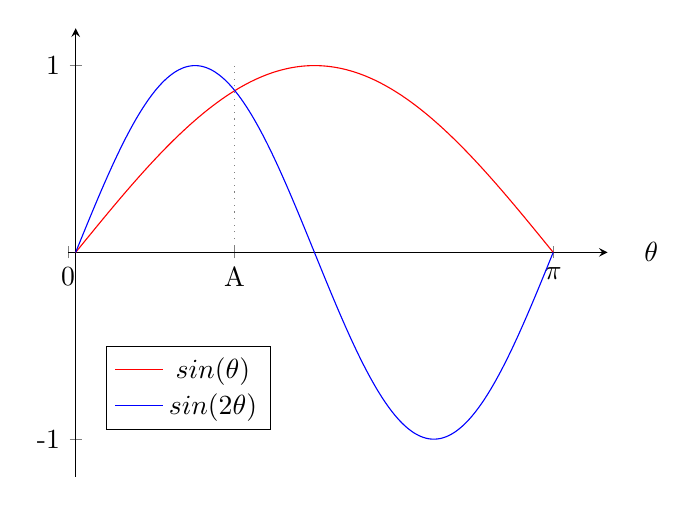
\begin{tikzpicture}\begin{axis}[axis lines=middle,samples=200
        ,xlabel=$\theta$
        ,ymax=1.2
        ,ymin=-1.2
        ,xmin = -0.05
        ,xmax = 3.5
        ,every axis x label/.style={
          at={(ticklabel* cs:1.05)},
            anchor=west,
          },
        every axis y label/.style={
          at={(ticklabel* cs:1.05)},
            anchor=south,
          },
        ,xtick=data
        ,xtick={-0.05,1.045,3.141592}
        ,xticklabels={0,A,$\pi$}
        ,ytick=data,
        ,ytick={1,-1}
        ,yticklabels={1,-1}
        ,legend style={at={(axis cs:0.2,-0.5)},anchor=north west}
        ]
      \addplot[red,domain=0:3.141592] {sin(deg(x)};
      \addplot[blue,domain=0:3.141592] {sin(deg(2*x))};
      \addplot[gray,dotted,mark=none] coordinates {(1.045, 0) (1.045, 1)};
      \legend{$sin(\theta$),$sin(2\theta$)}
\end{axis}\end{tikzpicture}
% \end{document}

  \caption{Dall'origine al punto A il comportamento di $\Im[\P]$ è induttivo, tra A e $\pi$ è capacitivo}
  \label{fig:capIndutt}
\end{figure}

\section{Parametri di un'antenna}\label{sec:paramAnt}
Mostreremo ora i parametri attraverso cui un'antenna è caratterizzata, prima elencandoli e poi ricavandoli per il dipolo elementare.
I parametri, dunque, sono
\begin{itemize}
  \item Pattern di radiazione in campo e in potenza
  \item SLL - Side Lobe Level
  \item Direttività
  \item Guadagno in potenza
\end{itemize}

\subsection{Pattern di radiazione}
\paragraph{Pattern di radiazione in campo}
Si definisce Pattern di radiazione in campo il rapporto
\begin{equation} \label{eq:patternCampo}
  F(\theta,\Phi) = \frac{E_\theta(r,\theta,\Phi)}{E_\theta(r,\theta_{max},\Phi_{max})}
\end{equation}
dove
\begin{equation}
  \{\theta_{max} , \Phi_{max}\} = \max_{\theta,\Phi} |E_\theta(r,\theta,\Phi)|
\end{equation}

Nel caso del dipolo elementare, si ha:

\begin{equation}
  F_{DE}(\theta,\Phi) = \frac{\jmath\eta I \frac{\Delta z}{\lambda} \frac{\ejbr}{r} sin(\theta)}{\jmath\eta I \frac{\Delta z}{\lambda} \frac{\ejbr}{r}} = sin(\theta) \, \theta_{max}=\frac{\pi}{2} \implies sin(\theta_{max}) =1
\end{equation}


\paragraph{Pattern di radiazione in potenza}
Definiamo il pattern di radiazione in potenza come
\begin{equation}\label{eq:patternPotenza}
  P(\theta,\Phi) = |F(r,\theta,\Phi)|^2 = \frac{|E_\theta(r,\theta,\Phi)|^2}{|E_\theta(r,\theta_{max},\Phi_{max})|^2} = \frac{|I|}{|I_{max}|} \, 0\le P(\theta,\Phi) \le 1
\end{equation}

Nel caso del dipolo elementare si ha che il pattern di radiazione in potenza è
$|  F_{DE}(\theta,\Phi)|^2 = sin^2(\theta)$

\subsection{Side Lobe Level SLL}
Definiamo il rapporto dei lobi secondari come
\begin{equation}\label{eq:SLL}
  SSL=10 \cdot log_{10}\left|\frac{F(SSL)}{F_{max}}\right|^2 = 20 \cdot log_{10} |F(SSL)|
\end{equation}
tenendo a mente che $F_{max}=1$

\paragraph{Solidi di direttività}
Dal pattern di radiazione in campo e in potenza, possiamo trovare i solidi di direttività in campo lontano. Il solido di direttività è un grafico tridimensionale che in coordinate sferiche permette di valutare la propagazione. Nel caso del dipolo elementare i suoi solidi di direttività in campo e in potenza sono visibili in figura \ref{fig:pattern}.
Poiché la maggior parte delle volte risulta difficoltoso rappresentare un grafico tridimensionale che sia facile e veloce da leggere, si decide di rappresentare un grafico bidimensionale, che verrà chiamato \textbf{diagramma di radiazione}.
Il diagramma di radiazione si costruisce omettendo uno dei due angoli $\theta$ o $\Phi$ e utilizzando
\begin{itemize}
  \item coordinate polari, la rappresentazione più utilizzata perché permette di cogliere immediatamente dove il campo si propaga;
  \item coordinate cartesiane, la rappresentazione che dà più risalto all'intensità del campo in determinati angoli.
\end{itemize}

\subsection{Direttività}
Il concetto di direttività di un'antenna è legato al voler quantificare la porzione di potenza che viene emessa nel lobo (o nei lobi) principali rispetto alla potenza media irradiata dall'antenna.
Iniziamo quindi a determinare come la potenza irradiata:
\begin{equation}
  P= \int_{S(r)} I(r,\theta,\Phi) dS =\int_0^\pi\int_0^{2\pi} I(r,\theta,\Phi)\cdot r^2 \cdot sin(\theta)d\theta\,d\Phi
\end{equation}

Definiamo quindi la potenza per unità di angolo solido la quantità
\begin{equation}
  U(\theta,\Phi)=I(r,\theta,\Phi)\cdot r^2 \quad [U] = W = \frac{W}{sterad}
\end{equation}
definiamo inolte il massimo della potenza per unità di angolo solido come:
\begin{equation}
  U_m = \max_{\theta,\Phi} U(\theta,\Phi) = U(\theta_{max},\Phi_{max})
\end{equation}
Possiamo quindi riscrivere la potenza come
\begin{equation}
  \int_0^\pi \int_0^{2\pi} U(\theta,\Phi) \cdot \underbrace{ sin(\theta) d\theta \, d\Phi}_{\text{ \parbox{2cm}{$d\Omega$ unità infinitesima di angolo solido}}}
\end{equation}
Da quest'ultima equazione possiamo definire la potenza media per unità di angolo solido come
\begin{equation}
  U_{AVG} = \frac{1}{4\pi}\cdot \int U(\theta,\Phi) \cdot d\Omega
\end{equation}
Definiamo quindi la direttivià come il rapporto
\begin{equation}
  D=\frac{U_m}{U_{AVG}}
\end{equation}

Possiamo riscrivere la direttività in due altri modi differenti:
\begin{esp}\label{eq:dirett}
  D&\stackrel{=}{1}\frac{I(r,\theta_{max},\Phi_{max})}{\frac{1}{4\pi}\int I(r,\theta,\Phi) sin(\theta) \cdot d\theta \, d\Phi} \\
  &\stackrel{=}{2}\frac{U_m}{\frac{P}{4\pi}} =\frac{U_m\cdot 4\pi}{P} = \frac{4\pi r^2 I(r,\theta_{max},\Phi_{max})}{P}
\end{esp}
La quantità $4\pi r^2 I(r,\theta_{max},\Phi_{max})$ viene normalmente chiamata \textbf{EIRP}: Effective Isotropic Radiated Power e indica un'antenna che trasmetta isotropicamente con un campo pari a quello nella direzione del massimo.

\paragraph{Direttività del dipolo elementare}

Nel dipolo elementare abbiamo che:
\begin{esp*}
  U(\theta,\Phi) &= \frac{\eta \cdot |I|^2}{8} \cdot \left(\frac{\Delta z}{\lambda}\right)^2 sin(\theta) \\
  U_m &= \frac{\eta \cdot |I|^2}{8} \cdot \left(\frac{\Delta z}{\lambda}\right)^2\\
  P&= \frac{\pi}{3}\eta |I|^2 \left(\frac{\Delta z}{\lambda}\right)^2 \\
  \implies & D_{DE} = \frac{U_m \cdot 4\pi}{P}= \frac{\frac{\eta \cdot |I|^2}{8} \cdot \left(\frac{\Delta z}{\lambda}\right)^2 \cdot 4\pi}{\frac{\pi}{3}\eta |I|^2 \left(\frac{\Delta z}{\lambda}\right)^2} = \frac{3}{2} = 1,5
\end{esp*}
Il risultato ottenuto mostra come il dipolo elementare sia poco direttivo. Spesso però si è soliti riportare la direttività in decibel rispetto a un'antenna isotropa (che quindi ha direttività pari a 1): $D_{DE_{dB}} \approx 1.76 dB$

Ipotizziamo ora un'antenna ideale che emette in un settore della sfera, per esempio supponiamo il pattern di radiazione in campo pari a:
\begin{equation}F=\begin{cases}
  1 & \frac{\pi}{3}\le \theta \le\frac{2}{3}\pi \\ 0 & \text{altrove}
\end{cases}\end{equation}
Possiamo scrivere la potenza media per unità di angolo solido come
\begin{equation}
  U_{AVG} =\frac{1}{4\pi}\int U(\theta,\Phi) d\Omega = \frac{U_m}{4\pi}\int |F|^2 d\Omega
\end{equation}

La direttività quindi risulta
\begin{esp*}
  D=\frac{U_m}{U_{AVG}} = 4\pi\frac{U_m}{U_m}\cdot \frac{1}{\int_0^{2\pi}\int_{\frac{\pi}{3}}^{\frac{2}{3}\pi} sin(\theta)d\theta \, d\Phi} = \frac{4\pi}{2\pi} = 2
\end{esp*}
Abbiamo quindi trovato un altro modo per scrivere $U(\theta,\Phi)$:
\begin{equation}
  U(\theta,\Phi) = |F(\theta,\Phi)|\cdot U_m
\end{equation}

Possiamo definire inoltre l'angolo solido del fascio, o \textit{beam solid angle} la quantità
\begin{equation}
  \Omega_A = \int |F(\theta,\Phi)|^2 d\Omega
\end{equation}
Otteniamo quindi che la direttività si può scrivere come
$$D= \frac{4\pi}{\Omega_A}$$.

\textsc{Remark:} a volte si scrive $D(\theta,\Phi) = D \cdot |F(\theta,\Phi)|^2$ rinormalizzando come visto in \eqref{eq:dirett} (2)
\subsection{Guadagno in potenza}
Non sempre si riesce a conoscere in ogni punto il valore di $I(r,\theta,\Phi)$, per cui si procede analizzando la potenza elettrica emessa rispetto alla direttività dell'antenna. In particolare, osservando anche la figura \ref{fig:antDipolo}, si procede come segue:
\begin{esp}
  P_{IN} &= \Re\left[\frac{V_A \cdot I_A^*}{2}\right] \\
  G= \frac{U_m}{\frac{P_{IN}}{4\pi}}
\end{esp}
Poiché si riesce sempre a calcolare
\begin{esp}
  4\pi U_m  &= G \cdot P_{IN} \leftrightarrow 4\pi U_m = D \cdot P\\
  \implies & G=D \frac{P}{P_IN} \quad D =G \frac{P_{IN}}{P}
\end{esp}
Sapendo che non esiste alcun materiale con resistenza nulla, si ha $P \le P_{IN}$. \\
Definiamo quindi efficienza dell'antenna o efficienza di radiazione la quantità
\begin{equation}\label{eq:efficienzaAnt}
  e_r = \frac{P}{P_IN}
\end{equation}

Possiamo ora riscrivere G come
\begin{esp*}
  G&=\frac{4\pi\U_m}{P_{IN}} \cdot \frac{r^2}{r^2} = \frac{4\pi r^2 I(r,\theta,\Phi)}{P_{IN}} = \frac{EIRP}{P_{IN}} \\
  EIRP &= G \cdot P_{IN} = D \dot P \\
  I(r,\theta,\Phi) &= G \frac{P_in}{4\pi r^2}\\
  \implies &G(\theta,\Phi) = G \cdot |F(\theta,\Phi)|^2
\end{esp*}

\section{Impedenza d'antenna}
Vogliamo ora valutare come adattare l'antenna affinché la maggior parte della potenza venga trasmessa e irradiata, invece che venir riflessa nel cavo.
Definiamo quindi l'impedenza di antenna:
\begin{equation}
  Z_A = \frac{V_A}{I_A} = R_A + \jmath \Chi_A
\end{equation}
dove $R_A$ è la resistenza d'antenna e $\Chi_A$ è la reattanza d'antenna.

Possiamo inoltre scrivere la potenza in ingresso all'antenna come:
\begin{esp*}
  P_{IN} &\stackrel{=}{1} \frac{R_A \cdot |I_A|^2}{2} = \Re\left[\frac{V_a \cdot I_A^*}{2}\right] \\
  &\stackrel{=}{2} \underbrace{P}_{pot. irradiata} + \underbrace{P_o}_{pot. dissipata}\\
  &= P + R_o \cdot \frac{|I_A|^2}{2}
\end{esp*}
definendo $R_o$ resistenza ohmica dell'antenna e $R_r$ la  resistenza di radiazione, tale per cui $P=R_r \cdot \frac{|I_A|^2}{2}$

Possiamo quindi ricavare
\begin{esp*}
  P_{IN} &= (R_o + R_r)\cdot \frac{|I_A|^2}{2}\\
  e_r &= \frac{R_r}{R_r + R_o} = \frac{R_r}{R_A} \le 1
\end{esp*}

Nel caso del dipolo elementare, supponendo una resistenza ohmica trascurabile, otteniamo:
\begin{esp}\label{eq:pot-resRadDE}
  P&=\frac{\pi}{3} \eta |I_A|^2 \cdot \left(\frac{\Delta z}{\lambda}\right)^2 \quad P_{IN} = P \\
  R_r &= \frac{2P}{|I_A|^2} = \frac{2}{3}\pi \eta \left(\frac{\Delta z}{\lambda}\right)^2 = 80\pi^2\left(\frac{\Delta z}{\lambda}\right)^2 \Omega
\end{esp}
Poiché il rapporto $\left(\frac{\Delta z}{\lambda}\right)$ è molto piccolo, l'antenna risulta poco efficiente.
Osserviamo ora la potenza reattiva emessa dall'antenna, in modo da calcolare $\Chi_A$. Iniziamo riprendendo l'equazione \eqref{eq:bilancio_potenza_EM_steinmetz}:
\begin{esp*}
  \Im\left[- \int_V \E \cdot \J^* ~ dV\right] &= \omega \underbrace{\int_V \omega \left[\mu \frac{|\H|^2}{2} - \epsilon \frac{|\E|^2}{2} \right] dV}
    _{<0} + \Im\left[\int_{S(r)} \P \cdot \hr dS\right] \\
  \Im\left[\frac{V_a \cdot I_A^*}{2}\right] &= -\omega\epsilon
\end{esp*}
Da quanto trovato in eq. \eqref{eq:campoEM}, sappiamo che $H_\Phi \propto \frac{1}{r^2}$ e $E_\theta \propto \frac{1}{r^3}$, dunque
\begin{esp*}
  \frac{\mu|\H|^2}{2} &\approx \frac{\mu}{r^2}\\
  \frac{\epsilon|\E|^2}{2} &\approx \frac{\mu}{r^6}\\
  &\stackrel{\implies}{r<1} \frac{\epsilon|\E|^2}{2} \gg \frac{\mu|\H|^2}{2}
\end{esp*}
Inoltre $\Im[\P]\approx 1$, per cui
\begin{esp*}
  \Im[\P] &= \frac{\eta}{3} |I_A|^2 \cdot \left(\frac{\Delta z}{\lambda}\right)^2 \cdot \Im[-\jmath] \left(\frac{\lambda}{2\pi r} \right)^3\\
  &= \frac{\eta}{3} |I_A|^2 \cdot \frac{\Delta z^2 \lambda}{8\pi^3 r^3} \ll -1
  & \implies \Chi_A \ll -1 ~  \text{negativo e molto grande}
\end{esp*}

\subsection{Adattamento dell'antenna}
Il segnale trasmesso da un'antenna proviene da un generatore collegato attraverso una linea (coassiale, bifilare o guida d'onda) che possiede una sua impedenza caratteristica. È quindi necessario adattare l'antenna, che considereremo come un dipolo elettrico, alla linea di trasmissione per ridurre le riflessioni e permettere che, al limite, tutta la potenza venga trasmessa.
Definiamo quindi impedenza caratteristica, la quantità
\begin{equation}
  Z_C = \frac{V+}{I_+} = \sqrt{\frac{l}{c}}
\end{equation}
Se la linea è priva di perdite, $Z_C \in \R$ e, in generale $Z_C = \{ \underbrace{50,75}_{\text{coassiale}} , \underbrace{100\div300}_{\text{\parbox{3cm}{linee bifilari}}}\} \Omega$

Definiamo ora il coefficiente di riflessione della linea:
\begin{equation}
  \rho = \frac{Z_A -Z_C}{Z_A + Z_C}
\end{equation}
dove $Z_A$ è l'impedenza d'antenna e $Z_C$ è l'impedenza caratteristica
Nel caso del dipolo elementare, dato che la reattanza è molto maggiore della resistenza e quest'ultima è molto piccola, possiamo scrivere:
\begin{esp*}
  |\rho| &\approx \frac{|\jmath \Chi_A -Z_C|}{|\jmath \Chi_A +Z_C|}\approx 1 \\
  P_{IN} = P(1-|\rho|^2) = \frac{|V_+|^2}{Z_C}(1-|\rho|^2) \approx 0
\end{esp*}
Se ho riflessione alta, l'antenna non irradia e tutto il segnale viene riflesso al generatore.

Bisogna quindi adattare l'antenna adottando una delle seguenti strategie:
\begin{itemize}
  \item modifico $Z_A$ in modo tale che sia simile a $Z_C$, ma spesso non è una cosa fattibile perché è legata al pattern di radiazione desiderato.
  \item utilizzo gli adattatori d'impedenza, che però hanno due principali limiti
  \begin{itemize}
    \item introducono perdite
    \item adattano l'antenna alla linea una banda limitata. Costruire adattatori a banda larga è più costodo e difficile da realizzare.
  \end{itemize}
\end{itemize}
Definiamo ora la matrice di scattering, una matrice quadrata di ordine N che rappresenta come avviene la diffusione di un segnale che entra in un N-polo.
Dato $a_i$ l'ingresso i-esimo e $b_i$ l'uscita i-esima, abbiamo
\begin{equation}
  \begin{cases}
    S_{ii} = \left. \frac{b_i}{a_i}\right |_{a_k = 0 \forall k \neq i} & \text{\parbox{3cm}{coefficiente di riflessione}} \\
    S_{ij} = \left. \frac{b_i}{a_j}\right |_{a_k = 0 \forall k \neq j} & \text{\parbox{3cm}{coefficiente di trasmissione}} \\
  \end{cases}
\end{equation}
In particolare, vogliamo che $S_{ii}\to0$, in modo che non ci sia riflessione.
\begin{esp*}
    P_{IN} = \frac{1}{2}\sum\limits_{i=1}^N |a_i|^2 - |b_i|^2 \stackrel{=}{conti}=\frac{1}{2} A^{*^T}\cdot D \cdot A
\end{esp*}

\section{Momento di dipolo equivalente }
Vogliamo ora cercare di estendere quanto calcolato per il dipolo elementare a qualsiasi antenna, valutando i casi in cui è possibile adottare le approssimazioni di campo lontano e in generale, quali sono le differenze con il caso studiato in precedenza.

Ipotizziamo ora un volume dove scorre una corrente impressa e che al di fuori del volume stesso ci sia un campo di radiazione. Calcoleremo quindi  il vettore $\M$ introdotto in eq. \eqref{eq:maxw-ant}.

Supponiamo che il vettore densità totale di corrente elettrica sia
\begin{equation}\J(\r\prime)=\begin{cases}
  \neq 0 & \forall r\prime \in V\prime \\ 0 & \text{altrove}
\end{cases}\end{equation}
Per ogni punto P si ha che il vettore posizione sia $\vec{R} = \vec{R}(\vec{r}\prime)$ dove $\vec{r}\prime$ è la distanza dal centro alla superficie del volume, in quanto siamo interessati a ogni contributo infinitesimo dalla superficie della sfera al punto P.

Il differenziale del potenziale vettore magnetco è
\begin{equation}
  d\A(\r) = \frac{\mu}{4\pi} \J(\r) \frac{e^{-\jmath \beta R}}{R}d\r\prime
\end{equation}

Possiamo quindi calcolare quanto vale $\A(\r)$
\begin{equation}
  \A(\r)=\int_{V\prime} d\A(\r) =\int_{V\prime} \frac{\mu}{4\pi} \J(\r) \frac{\ejbr}{R}d\r\prime
\end{equation}
Cerchiamo ora di trovare una maniera più semplice per trovare $R=|\vec{R}(\r\prime)|$
\begin{esp}
  R&=|\vec{R}(\r\prime)| = \sqrt{r^2+r\prime^2-2r\cdot r\prime cos(\psi)} \\
  &= r\cdot \sqrt{1+\left(\frac{r\prime}{r}\right)^2-2\frac{r\prime}{r} cos(\psi)} = r \cdot\sqrt{1+\Delta} \\
  &\approx r \cdot \left(1+\frac{\Delta}{2} + o\left( \left( \frac{r\prime}{r} \right)^2 \right) \right)\\
  \Delta &= -2\frac{r\prime}{r} cos(\psi)+\left(\frac{r\prime}{r}\right)^2 \approx -2\frac{r\prime}{r} cos(\psi)+o\left[\left(\frac{r\prime}{r}\right)^2\right]
\end{esp}

Possiamo quindi scrivere $\A(\r)$ come:
\begin{esp*}
  \A(\r)&\approx \int_{V\prime} \frac{\mu}{4\pi} \J(\r) \frac{e^{-\jmath\beta \cdot[r-r\prime cos(\psi)]}}{r}d\r\prime
\end{esp*}
dove il denominatore è potuto essere approssimato a $r$ perché non ha un cambiamento significativo al risultato dell'integrale, mentre nell'esponenziale il termine di fase avrebbe comportato un cambiamento molto maggiore, per cui non si può applicare alcuna semplificaizione.\\
Continuando con i conti, otteniamo
\begin{esp*}
  \A(\r) &= \underbrace{\frac{\mu\ejbr}{4\pi r}}_{\text{onda sferica}} \cdot \int_{V\prime}\J(\r\prime)\cdot e^{-\jmath\beta r\prime cos(\psi)} dr\prime \\
  &=\frac{\mu \ejbr}{4\pi r} \cdot \M(\theta,\Phi)\\
\end{esp*}
Abbiamo quindi trovato che il momento di dipolo equivalente vale
\begin{equation}
  \M(\theta, \Phi) = \int_{V\prime}\J(\r\prime)\cdot e^{-\jmath\beta r\prime cos(\psi)} dr\prime
\end{equation}

L'approssimazione vale
\begin{esp}
  &r \cdot \left(1+\frac{\Delta}{2} + o\left[ \left( \frac{r\prime}{r} \right)^2 \right]\right) \approx r-r\prime cos(\psi) + \underbrace{\frac{r\prime^2}{r}}_{\ll 1} \\
  &\beta \frac{r\prime^2}{r} \ll 1 \Leftrightarrow \frac{2\pi }{\lambda}\frac{r\prime^2}{r} \ll 1\Leftrightarrow \frac{2\pi D^2}{\lambda r} \ll 1 \\
  & 2 \pi \underbrace{\frac{D}{\lambda}}_{(1)}\underbrace{\frac{D}{r}}_{(2)}
\end{esp}
dove $(1)$ considera il rapporto tra la dimensione dell'antenna e lunghezza d'ona, mentre $(2) \ll 1$  perché considero il campo lontano.

Le condizioni di campo lontano sono valide:
\begin{itemize}
  \item $r\gg \lambda$ per il dipolo elementare e le antenne filiformi
  \item $r\gg \frac{D^2}{\lambda}$
\end{itemize}

\subsection{Altezza efficace}
Definiamo altezza efficace in trasmissione
\begin{equation}
  \h_T(\theta,\Phi) t.c. \E= \jmath \frac{\eta}{2\lambda} \frac{\ejbr}{r}\h_T(\theta,\Phi I_A)
\end{equation}
Nel caso del dipolo elementare $\h_T(\theta,\Phi) = \Delta z \hz$

Cerchiamo ora di definire l'altezza efficace in ricezione. Presupponiamo di adattare il carico $Z_A=Z_C=Z_G$. Supponiamo inoltre che $\E_i$ sia il campo elettrico incidente sull'antenna determinato in assenza dell'antenna stessa. L'antenna si può quindi schematizzare come in figura \#TODO.

Possiamo inoltre scrivere, definita $\h_R$ l'altezza efficace in ricezione
\begin{equation}
  V_G=\E_i \cdot \h_R^*(\theta,\Phi)
\end{equation}

La potenza al ricevitore sarà quindi:
\begin{equation}
  P_R=\Re\left[\frac{V_L \cdot I_L^*}{2}\right] = \frac{|V_G|^2}{2} \cdot \frac{R_L}{|Z_L+Z_A|^2} =\frac{R_L \cdot |\E_i \cdot \h_R^*|^2}{2\cdot|Z_L+Z_A|^2}
\end{equation}
Per il teorema di reciprocità possiamo scrivere che
\begin{equation}
  \h_T(\theta,\Phi) = \h_R(\theta,\Phi)
\end{equation}
Inoltre otteniamo che se
\begin{equation}
  \E_i \cdot \h_R^* =0 \implies \E_i \perp \h_R
\end{equation}
ossia sono a polarizzazione ortogonale.
Definiamo quindi l'adattamento di polarizzazione
\begin{equation}
  p=\frac{|\E_i \cdot \h_R^*|^2}{|\E_i|^2 \cdot |\h_R|^2} ~ p \in [0;1]
\end{equation}

Nel caso in cui $\E_i \cdot \h_R^* = \gamma |\h_R|$ allora $\E_i \parallel \h_R$ e $p=1$. Possiamo riscrivere
\begin{equation}
  p= \left|\frac{\E_i}{|\E_i|}\cdot\frac{\h_R}{|\h_R|}\right| = |\hat{e}_i \cdot \hat{h}_R^*|^2
\end{equation}
in cui $\hat{e}_i$ e $\hat{h}_R^*$ sono i fasori di direzione.

Le antenne trasmittente e ricevente possono essere rappresentate come due dipoli di lunghezza $\h_x,\h_y$ e tensioni $V_x,V_y$. In particolare possiamo scrivere:
\begin{equation}\begin{cases}
  \h_x = \Delta l \cdot \hat{x} & V_x = E_x \cdot \Delta l \\
  \h_y = \Delta l \cdot \hat{y} & V_y = E_y \cdot \Delta l
\end{cases}\end{equation}
Nella linea, in posizione $-\frac{\lambda}{4}$ otteniamo
\begin{esp}
  V_y(-\frac{\lambda}{4}) &= V_y \cdot e^{\jmath \beta \frac{\lambda}{4}} = E_y \cdot \Delta l \cdot e^{\jmath \frac{2\pi}{\lambda}\frac{\lambda}{4}} = \jmath E_y \Delta l \\
  V&= V_x + V_y(-\frac{\lambda}{4}) = E_x \Delta l+\jmath E_y \Delta l = \left(\underbrace{E_x \cdot \hat{x} E_y \cdot \hat{y}}_{\E}\right) \cdot \Delta l \cdot \left(\underbrace{\hat{x} + j\hat{y}}_{\h_R}\right)
\end{esp}
Possiamo quindi esprimere $\h_R = \left(\hat{x} + j\hat{y}\right)$. In generale possiamo ricevere un'onda con polarizzazione circolare destrorsa, mentre si annulla la polarizzazione circolare sinistrorsa.
Un'onda polarizzata linearmente, inoltre, se entra in un'antenna a polarizzazione circolare porta metà potenza dell'antenna stessa. Questa cosa viene sfruttata nelle comunicazioni tra le stazioni radio base (BTS) e i cellulari.
La potenza al ricevitore risulta:
\begin{esp*}
  P_R &= \frac{R_L}{2|Z_A+Z_L|^2}\frac{|\E_i \cdot \h_R^*|^2}{|\E_i|^2 \cdot |\h_R|^2} \cdot |\E_i|^2 \cdot |\h_R|^2\\
  &=\frac{R_L}{2|Z_A+Z_L|^2} \cdot p \cdot \cdot |\E_i|^2 \cdot |\h_R|^2
\end{esp*}

\paragraph{Esempio GNSS}
Nel caso di navigazione satellitare, sistemi come il GPS, il GLONASS, Beidou e IRNSS utilizzano una polarizzazione circolare destrorsa, in quanto l'onda, dopo una riflessione, inverte il verso di polarizzazione e si attenua leggermente. L'antenna del cellulare, quindi, filtra naturalmente una riflessione.In caso di doppia riflessione su materiale non conduttore il segnale è molto più attenuato, per cui verrà considerato come rumore di fondo. Il problema si verifica in caso di doppia riflessione su buon conduttore.
Le equazioni che lo legano sono riportate qui:
\begin{esp*}
  \E_i &= (E_x \cdot \hat{x}+E_y \cdot \hat{y}) \cdot e^{\textcolor[rgb]{0.8,0,0}{-}\jmath \beta z} \\
  \E_r &= (E_x \cdot \hat{x}+E_y \cdot \hat{y}) \cdot \rho \cdot e^{\textcolor[rgb]{0.8,0,0}{+}\jmath \beta z} \\
\end{esp*}
\subsection{Area efficace}
Definiamo area efficace di un'antenna il rapporto:
\begin{equation}\label{eq:Aeff}
  A_{e_m}=\frac{P_{R_{max}}}{I_i(r,\theta,\Phi)} \quad [A_{e_m}] = m^2
\end{equation}

dove $I_i$ è l'intensità di radiazione nel punto dove si inserisce l'antenna, in assenza dell'antenna stessa.
\subsection{Ottimizzazione della potenza ricevuta}
La potenza ricevuta dipende
\begin{equation}\begin{cases}
  \text{Dal carico $(R_L,Z_L)$} \\
  \text{Dalla polarizzazione (relativa fra $\E_i,\h_R$)}
  \text{Dall'orientamento dell'antenna ricevente ($\h_R$)}
\end{cases}\end{equation}
Nel caso del dipolo elementare
\begin{equation}
  \E = \jmath \frac{\eta}{2\lambda} \cdot \frac{\ejbr}{r} \cdot \underbrace{\Delta z \cdot sin(\theta) \hth}_{\h_r(\theta,\Phi)}
\end{equation}
Per il teorema di reciprocità se l'antenna trasmette bene in una direzione, riceverà bene nella stessa direzione. Per massimizzare la potenza al ricevitore, devo supporre:
\begin{enumerate}
  \item Adattamento in potenza: in figura \ref{fig:antRic} $Z_A=Z_L^*$
    \begin{figure}
%      \includegraphics{}
      \caption{L'antenna è schematizzata come generatore, la sua resistenza è $Z_A$ e l'impedenza del carico collegato è $Z_L$}
      \label{fig:antRic}
    \end{figure}
    \begin{equation}
      Z_A=Z_L^* \implies \frac{R_L}{2|Z_A+Z_L|} =\frac{R_A}{2 \cdot 4\Re[Z_A]^2 } = \frac{1}{(R_A)}
    \end{equation}
  \item adattamento in polarizzazione: $p=1$
  \item orientamento ottimale dell'antenna in ricezione $|\h_R|=|\h_{R_{max}}|$
\end{enumerate}
Sotto queste tre condizioni
\begin{equation}\label{eq:PRmax}
  P_{R_{max}} = \frac{|\E_i|^2 \cdot |\h_R|^2}{8 R_A} = I(r,\theta,\Phi)\cdot A_{e_{max}}
\end{equation}

\subsection{Regime di campo lontano}
In regime di campo lontano possiamo assumere l'onda sferica, come onda piana uniforme. L'intensità di radiazione, l'area efficace massima e l'altezza efficace risultano
\begin{esp}
  I_i(r,\theta,\Phi) &= \frac{|\E_i|^2}{2\eta} \\
  A_{e_{max}} &= \frac{\eta}{4 R_A} \cdot |\h_{R_{max}}|^2 \\
  |h_{R_{max}} &= 2 \sqrt{\frac{R_A \cdot A_{e_{max}}}{\eta}}
\end{esp}
\paragraph{Caso dipolo elementare}
\begin{esp}
  |h_{R_{max}} &= \Delta z^2\\
  R_A=R_r=2 \frac{2}{3}\pi\eta\left(\frac{\Delta z}{\lambda}\right)^2\\
  A_{e_{max}} &= \frac{\eta\cdot\Delta z^2}{4 \frac{2}{3}\pi\eta\left(\frac{\Delta z}{\lambda}\right)^2}= \frac{3}{8\pi} \lambda^2 \\
\end{esp}
Poiché l'area efficace non dipende dalle dimensioni dell'antenna, è molto difficile adattare il sistema per ottenere $A_{e_{max}}$.

\subsection{Relazione tra i parametri di antenna in TX e RX}
Definiamo ora i parametri d'antenna come l'EIRP e la relazione tra area efficace, direttività, guadagno e efficienza di radiazione, prima in generale e poi nel caso del dipolo elementare
\begin{esp}
  EIRP &= 4\pi U_m = D \cdot P \quad \text{in trasmissione}\\
  &= 4\pi \cdot r^2 \cdot I(r,\theta_{max},\Phi_{max}) = D \cdot P \\
  &= \frac{|\E_{i_{max}}|^2}{2\eta}\cdot 4\pi \cdot r^2 =D \cdot P = D \cdot R_r \frac{|I_A|^2}{2} \\
  &= \frac{\eta \pi |I_A|^2}{\lambda^2} \cdot |\h_{max}|^2 = D\cdot R_r \cdot |I_A|^2 \\
  \Leftrightarrow &\frac{\eta \pi}{\lambda^2} \cdot |\h_{max}|^2 = D\cdot R_r
  \implies & \frac{\eta \pi |I_A|^2}{\lambda^2}\frac{4 R_A}{\eta} \cdot A_{e_{max}} = D\cdot R_r
\end{esp}
Supponendo di non avere perdite ($R_o = 0$), si ottiene che per qualsiasi antenna
\begin{equation}\label{eq:rapportoParam}
  \frac{A_{e_{max}}}{D} = \frac{\lambda^2}{4\pi}
\end{equation}

Verifichiamo ora il rapporto appena ricavato nel caso del dipolo elementare:
\begin{esp*}
  D&=\frac{3}{2} \quad A_{e_{max}}=\frac{3}{8\pi}\cdot \lambda^2 \implies \frac{A_{e_{max}}}{D} =\frac{\frac{3}{8\pi}\cdot \lambda^2}{\frac{3}{2}}  = \frac{\lambda^2}{4\pi}
\end{esp*}
Le antenne reali presentano delle perdite, per cui utilizzo il guadagno. Ottengo quindi:
\begin{esp*}
  G&=e_r \cdot D \quad A_e = e_r \cdot A_{e_{max}} \text{ area efficace}\\
  \frac{A_{e_{max}}}{D} &= \frac{e_r \cdot A_{e_{max}}}{e_r \cdot D }=\frac{A_e}{G}=\frac{\lambda^2}{4\pi} \\
  \implies &\frac{A_e}{G}=\frac{\lambda^2}{4\pi} \\
\end{esp*}
\section{Dimensionamento di TX di potenza (formula di Friis)}
Affinché si possa applicare la formula di Friis, che risulta comoda per calcolare la potenza al ricevitore, sono necessarie le seguenti condizioni:
\begin{enumerate}
  \item Antenne sono in campo lontano, ossia
  \begin{equation*}\begin{cases}
    d\gg \lambda & \text{se } D \ll \lambda \\
    d \gg \frac{2D^2}{\lambda} & \text{se } D\ge 2,5\lambda
  \end{cases}\end{equation*}
  \item Adattamento in potenza di $Z_L$ e adattamento alla linea $Z_C$
  \item Adattamento in polarizzazione dell'antenna riceventa
  \item Orientamento ottimale di entrambe le antenne
\end{enumerate}
Sotto queste condizioni possiamo scrivere
\begin{esp*}
  EIRP&= G_{TX}\cdot P_{IN}\\
  \frac{|\E_{i_{max}}|^2}{2\eta}\cdot 4\pi \cdot d^2 &= G_{TX}\cdot P_{IN} \\
  \frac{|\E_{i_{max}}|^2}{2\eta} &= \frac{G_{TX}\cdot P_{IN}}{4\pi d^2}\\
  P_{R_{max}} &= \frac{|\E_{i_{max}}|^2}{2\eta} \cdot A_{e_{max}}^{RC} = \frac{G_{TX}\cdot P_{IN}}{4\pi d^2}\cdot \frac{\lambda^2}{4\pi}\cdot G_{RC}
\end{esp*}
Si ottiene quindi la \textbf{formula di Friis}:
\begin{equation}\label{eq:friis}
  P_{R_{max}} = G_{TX}\cdot G_{RC}\cdot P_{IN}\cdot \left(\frac{\lambda}{4\pi d}\right)^2
\end{equation}
